\section{Discrete Wavelet Transform}

\subsection{One dimensional DWT}

\begin{figure}
    \centering
    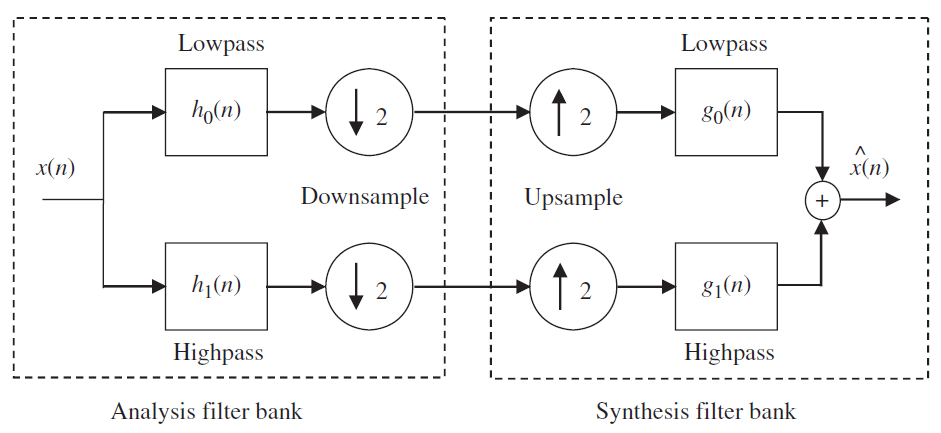
\includegraphics[scale=0.5]{dwt_1d_anal_synth.png}
    \caption{1-D DWT, two-band wavelet analysis and synthesis filter banks \cite{jpeg_suite}}
    \label{fig:dwt_1d_anal_synth}
\end{figure}

The linear convolution (filtering) of sequences $x(n)$ and $h(n)$ is defined as in equation \ref{eq:convolution}:
\begin{equation}
    y(n)=\sum_{m=-\infty}^{\infty}x(m)h(n-m)
\label{eq:convolution}
\end{equation}
The one dimensional discrete wavelet transform can be depicted as successive applications (convolutions) of
one seleceted pair of high and low-pass filters. The output of such application is then followed
by downsampling by the factor of two. For example, it can be achieved by discarding samples with
odd indices after each of filtering operation. It is better visualized in the Figure \ref{fig:dwt_1d_anal_synth}. \cite{jpeg_suite} 
The pair of low and high-pass filters is known as analysis filter bank in the encoding process.
In the signal decoding process it is featured as a synthesis filter bank. The decoding step requires
using the inverse of discrete wavelet transform. 

Take into consideration a one dimensional signal $x(n) = \{55, 234, 70, 21, 88, 37\}$. It can be better
understood as values of pixels in a part of the grayscale image row. It is followed with a pair of low
and highpass filters designated by $h_{0}(n)$ and $h_{1}(n)$ respectively. An example of such pair is
a lowpass filter $h_{0}(n) = \{-1, 2, 6, 2, -1\}/8$ and a highpass filter $h_{1}(n) = \{-1, 2, -1\}/2$. They are both
symmetric and consist of only integer taps. Such pair can be presented in the notaion of (5, 3) filter bank.
This convension indicates that the length of lowpass filter is five and the length of highpass filter is three.
In fact the analysis fitler bank presented here was firstly proposed by LeGall and Tabatabai in 1988 and
is used in the JPEG 2000 standard for lossless compression of images. The filtering operation has to
be defined at the signal boundaries. Therefore, the one dimensional signal is extended in both directions.
The Part 1 of the JPEG 2000 standard requires symmetrical extension to be perfomed in such case. \cite{jpeg_suite}
After applying the required symmetrical padding the signal is extended to
$x(n) = \{21, 70, 234, 55, 55, 234, 70, 21, 88, 37, 37, 88, 21, 70\}$. Then, the lowpass fitler is applied
resulting in $x'_{0}(n) = \{197.25, 75.5, 98.375, 67.125, 45.375\}$ and the higpass one which results in
$x'_{1}(n) = \{44.75, -85.75, 29, 12.75, -29.5\}$.

\begin{figure}
    \centering
    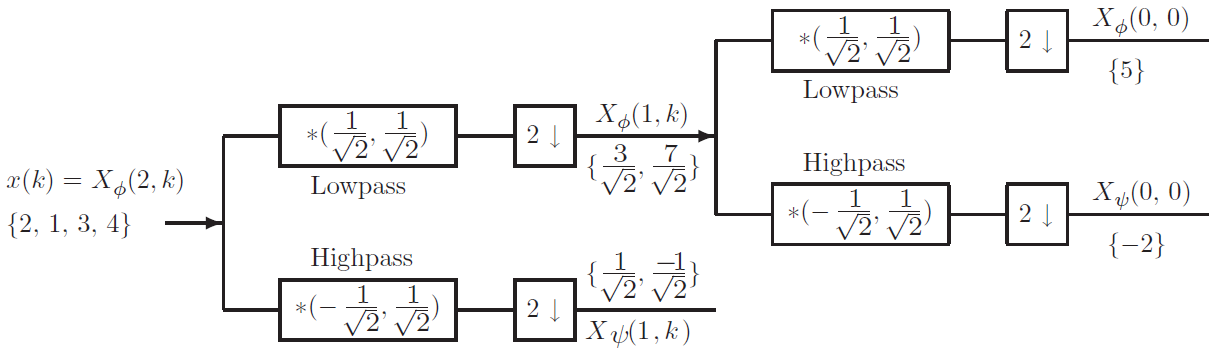
\includegraphics[scale=0.45]{dwt_1d_2_level.png}
    \caption{Computation of a 2-level 4-point DWT using a two-stage two-channel Haar analysis filter bank \cite{dwt_impl}}
    \label{fig:dwt_1d_2_level}
\end{figure}

The next example shows how to compute the two levels of discrete wavelet transform. To speed up the process
no padding option is chosen this time which makes it non-compliant with the JPEG 2000 standard.
The filter used here is the most basic one, i.e. Haar analysis filter bank. It is the first wavelet
from the Daubechies wavelet family. The calculation process is visualized in the Figure \ref{fig:dwt_1d_2_level}. \cite{dwt_impl}

The input is chosen as 4-point signal $X_{\phi}(2, k) = \{2, 1, 3, 4\}$. This notaion emphasizes the fact
that it is approximation of the input at scale 2. The so called scalling coefficients (or in other term
approximation at scale 1) $X_{\phi}(1, k)$ are computed by convolving the input $x(k)$ with the low-pass
Haar filter impulse response $l(k) = \{1/\sqrt{2}, 1/\sqrt{2}\}$. In the next step there is downsampling
by a factor of 2 applied. The output of convolution has five values. The middle three from these fives 
correspond to cases where both the given input values overlap with the impuse response. As it was described
earlier, the odd values are preserved in the downsampling process. In a result first and third value of these
three middle ones are the approximation output $X_{\phi}(1, k)$. In the similar way, the detail coefficients
at scale 1 $X_{\psi}(1, k)$ are computed. The input $x(k)$ is convoled with the high-pass filter impulse
response $h(k) = \{-1/\sqrt{2}, 1/\sqrt{2}\}$. Then the downsampling by factor of 2 is perfomed.
Note that only only approximation output $X_{\phi}(1, k)$ of the first stage goes to the second one.
The $X_{\phi}(0, 0)$ and $X_{\psi}(0, 0)$ are calculated accordingly at the end of the second stage. \cite{dwt_impl}

\subsection{Two dimensional DWT}

The idea of using lowpass filter is the preservation of low frequencies of a signal while trying
to eliminate or at least attenuate the high frequencies. In a result the output signal is the blurred
version of the original one. Therefore, the operating principle of the highpass filter is completely
opposite. As a result of applying such filter, the high frequencies of the signal are preserved and
the low ones are discarded or at least dimnished. The output is a signal consisting of edges, textures
and other details. \cite{jpeg_suite} 

\begin{figure}
    \centering
    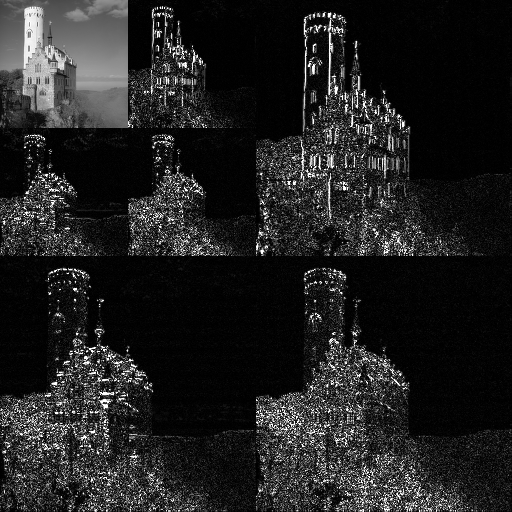
\includegraphics[scale=0.7]{dwt_2d_example_wiki.png}
    \caption{2D DWT applied 2 times to an exemplary image \cite{dwt_example_wiki}}
    \label{fig:dwt_2d_example_wiki}
\end{figure}

There is presented an example of the effects of the two dimensional discrete wavelet transform on the Figure \ref{fig:dwt_2d_example_wiki}.
The DWT used here is compliant with the Part 1 of the JPEG2000 standard. The number of DWT stages presented in this  
example is equal to two. Two dimensional discrete wavelet transform applied first time to the original image
yields four same sized subimages. The LL layer (upper left subimage) is an approximation of the image and contains the low frequencies.
This layer is once more transformed in the next stage. The LH layer (upper right subimage) preserves high frequencies from the rows of the image.
As a result vertical lines and details (brightness) can be seen in the produced subimage. On the other hand, the HL layer (bottom left)
contains high frequencies from the columns of the image. The horizontal details and lines can be noticed there.
Lastly, the HH layer (bottom right) preserves the diagonal lines. \cite{dwt_example_wiki}

\begin{figure}
    \centering
    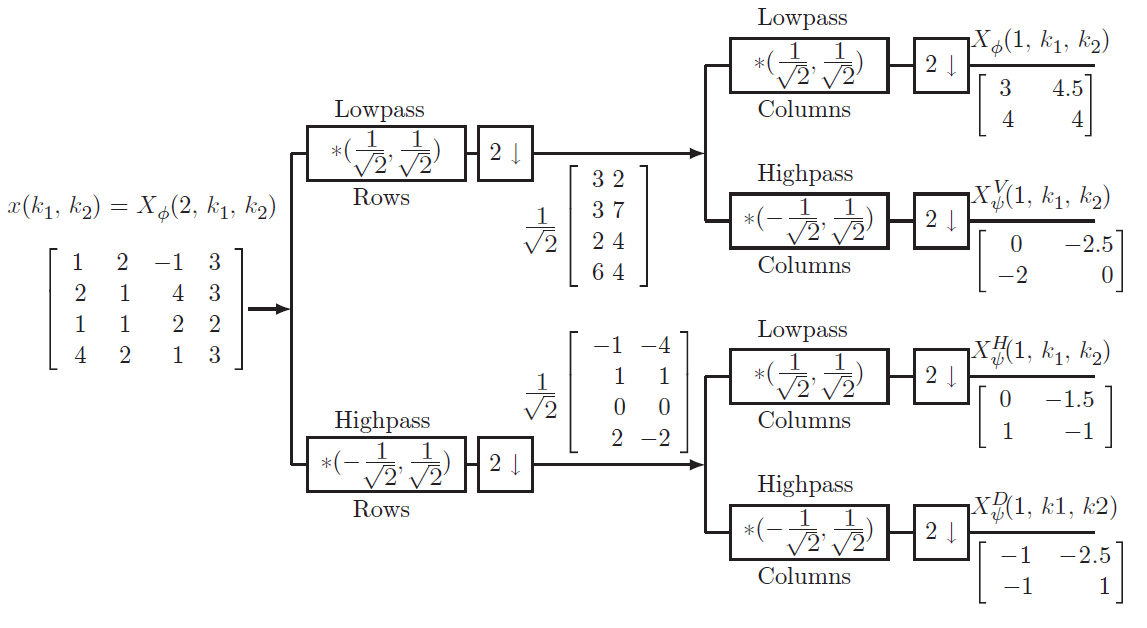
\includegraphics[scale=0.45]{dwt_2d_1_level.png}
    \caption{Computation of a 1-level 4 $\times$ 4 2-D Haar DWT using a two-stage filter bank \cite{dwt_impl}}
    \label{fig:dwt_2d_1_level}
\end{figure}

The process of computing a 1 level two dimensional discrete wavelet transform with usage of
two-stage analysis Haar filter bank is shown in Figure \ref{fig:dwt_2d_1_level}. Coefficients $\mathbf{X}_{\phi}$
are calculated as a result of lowpass filtering and downsampling to each row of the two dimensional
data. Next, similar process process, i.e. lowpass convolution and downsampling is applied to each column of
resulting data. The rest of coefficients is obtained in very similar fashion to the previous ones.
Coefficients $\mathbf{X}^{H}_{\psi}$ are calculated by applying high-pass filtering and downsampling to each row of the
2-D data $\mathbf{x}$ and then followed by applying sequence of low-pass filtering and downsampling to each
column of the resulting data. Coefficients $\mathbf{X}^{V}_{\psi}$ are obtained by applying low-pass filtering
and then downsampling to each column of the resulting data. Lastly, coefficients $\mathbf{X}^{D}_{\psi}$ are
obtained by applying hig-pass filtering and downsampling to each row of the 2-D data $\mathbf{x}$ followed by
applying highpass filtering and downsampling to each column of the resulting data. In the next stage of more
complex dwt calculating process only the coefficients $\mathbf{X}_{\phi}$ are taken into consideration. \cite{dwt_impl}

\subsection{DWT features summary}

\begin{itemize}
    \item In a nutshell, the discrete wavelet transform is a set of bandpass filters. Usually it is implemented
    with the usage of low and high-pass filters recursively.
    \item The computational complexity of computing the DWT in the best case is linear, i.e. $O(N)$.
    \item The first approach to implement the DWT efficiently is evaluation of the required convolutions
    with the usage of the polyphase filter structure.
    \item The second approach is factorization of the polyphase matrix into a product of a set of sparse matrices.
    \item The two dimensional discrete wavelet transform (with separable filters) is usually computed by the row-column method.
    One dimensional DWT of all the columns is computed at first. Then the 1-D DWT of all the resulting
    rows is calculated. The order of the computation does not matter in terms of achieving the same result.
    \item Additional memory of approximate half the size of the given data is required in the implementation of the DWT.
    \item Data reordering is required for an in-place computation of the DWT.
    \item Data expansion problem can occur due to the finite length of the data in the implementation of the asymmetric filters.
    \item Symmetric filters provide linear phase response and an effective solution to the border problem. \cite{dwt_impl}
\end{itemize}

\section{Part 2 of the JPEG 2000}

% Part2 in details
% write down different filters and basic ones

\subsection{Introduction}

Many ideas have been emerging as the JPEG 2000 was developed. These concept were full of
value-added capabilities. However, they were not that important to be gone through the time-consuming
ISO standardization process. The Part 1 (ISO/IEC, 2004a) of the standard, i.e. Core coding system, 
was originally published in 2000. There was a need to created additional parts to include
missing features. The Part 2 of the standard, published as ISO/IEC 15444-2 or ITU Recommendation
T.801 (ISO/IEC, 2004b), contains multiple such extensions. There is present group of rather small
additions that could not merit entire documents of their own. In the Part 1 Core of JPEG 2000
standard decoders are supposed to handle all of the code-stream functionality. The Part 2
is different from first one in this aspect. It is a collection of options that can be
implemented on demand to meet very specific requirements of the given market. Moreover,
sections within an extension annex can be implemented separately. For example, subsets
of extended file format JPX can be used on their own. Therefore, some features of the Part 2
may be present in the wide spectrum of JPEG 2000 applications while the other ones can be
less common in the decoders. \cite{jpeg_suite}

As it was shown in the previous paragraph, the extensions present in the Part 2 consist of 
very different set of topics that can modify or add some features to the Part 1 JPEG 2000 compliant 
processing chain. Some tools can result in the compression efficiency improvement. Others can
ameliorate the visual appearance of compressed images. Another group of extensions can modify
or extend some functionalities in the other ways. The list of the major topics is presented below. \cite{jpeg_suite}
\newline \newline Compression efficiency:
\begin{itemize}
    \item Variable DC offset (VDCO) - Annex B
    \item Variable scalar quantization (VSQ) - Annex C
    \item Trellis coded quantization (TCQ) - Annex D
    \item Extended visual masking - Annex E
    \item Arbitrary wavelet decomposition - Annex F
    \item Arbitrary wavelet transform kernel - Annexes G and H
    \item Multiple component transform - Annex J
    \item Nonlinear point transform - Annex K \cite{jpeg_suite}
\end{itemize}
\hfill \break Functionalities:
\begin{itemize} 
    \item Geometric manipulation - Annex I
    \item Single-sample overlap (SSO/TSSO) - Annex I
    \item Precinct-dependent quantization - Amendment 1
    \item Extended region of interest - Annex L
    \item Extended file format/metadata (JPX) - Annexes M and N
    \item Extended capabilities signaling - Amendment 2 \cite{jpeg_suite}
\end{itemize}

\subsection{Arbitrary Decomposition}

In the Part 1 of the JPEG 2000 standard there is only one wavelet decomposition structure allowed.
This wavelet is called Mallat dyadic decomposition. Such decomposition is a good first choice
to be applied across a wide spectrum of images. However, other ones can improve the quality of the image
over specialized classes of the applications. The other effect of applying such decompositions are
unequal reductions in the horizontal and vertical dimensional of reduced resolution extracts. \cite{jpeg_suite}

\begin{figure}
    \centering
    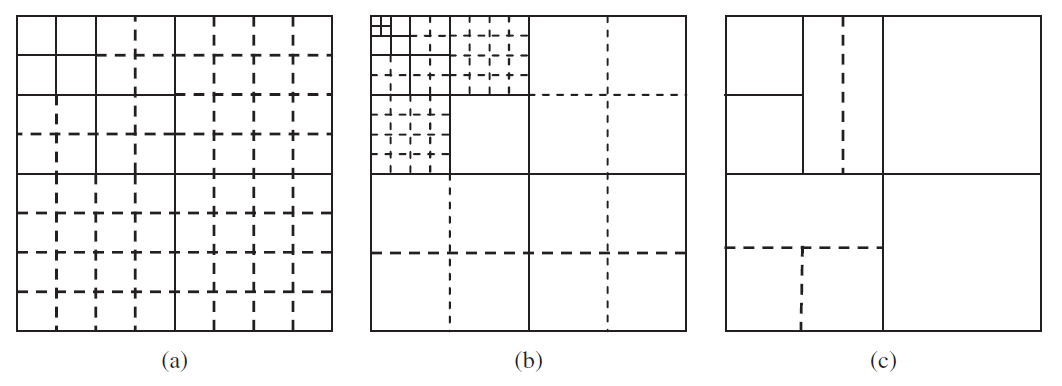
\includegraphics[scale=0.45]{part_2_decomp_examples.png}
    \caption{Some examples of decomposition compliant with the Part 2 \cite{jpeg_suite}}
    \label{fig:part_2_decomp_examples}
\end{figure}

Other decomposition styles can be found in the wavelet literature. They include the full packet
tree processing and some of its derivatives. The applied packet decomposition derivatives
can outperform the solution from Part 1 of the JPEG 2000 standard in some applications.
For instance, they come crucial at maintaining regular fine-grain texture. Moreover,
the applications that require processing synthetic aperture radar images can benefit
from using this extension. The US Federal Bureau of Investigation actively uses a 500 ppi
fingerprint compression standard, i.e. WSQ (CJIS, 1997). The decomposition is specialized
for the characteristics of fingerprint imagery at 500 dpi. \cite{jpeg_suite}

Some of these decomposition can be seen of the Figure \ref{fig:part_2_decomp_examples}.
Resolution decomposition is depicted as solid lines. Dashed lines represent extra sublevel
decomposition. On the first example, i.e. image $(a)$, there is available full packet decomposition
with such parameters: NL = 3: Ddfs = 111, Doads = 321, Dsads = all 1s. The next picture
illustrates FBI decomposition wit specified parameters: NL = 5: Ddfs = 11111, Doads = 2321,
Dsads = 11101111111111111. The last image is juts an arbitrary example. \cite{jpeg_suite}

The prespecified decomposition structures are not the only feature of this extension.
Wavelet packet analysis can be also used to design custom decompositions for specific images
or some types of images. It was implemented in Coifman and Wickerhauser, 1992; Ramchandan
anad Vetterli, 1993; Meyer, Averbuch, and Stromberg, 2000. Such applications often start with
a large decomposition tree. Then, they tend to locate a good decomposition based upon
specified optimization metric. \cite{jpeg_suite}

\subsection{Arbitrary Wavelet Transforms}

\begin{table}
    \centering
    \caption{Analysis and synthesis filter taps for the floating-point Daubechies (9, 7) filter bank}
    \label{tab:anal_synth_97i}
\begin{tabular}{ccc}
    \toprule
    n         & Lowpass, $h_{0}(n)$ & Lowpass, $g_{0}(n)$ \\
    \midrule
    $0$       & +0.602949018236360  & +1.115087052457000  \\
    $\pm 1$   & +0.266864118442875  & +0.591271763114250  \\
    $\pm 2$   & -0.078223266528990  & -0.057543526228500  \\
    $\pm 3$   & -0.016864118442875  & -0.091271763114250  \\
    $\pm 4$   & +0.026748757410810  &                     \\
    \bottomrule
\end{tabular}

\bigskip
\bigskip


\begin{tabular}{cc}
    \toprule
    n         & Highpass, $h_{1}(n)$ \\
    \midrule
    $-1$      & +1.115087052457000   \\
    $-2, 0$   & -0.591271763114250   \\
    $-3, 1$   & -0.057543526228500   \\
    $-4, 2$   & +0.091271763114250   \\
              &                      \\
    \bottomrule
\end{tabular}
\quad
\begin{tabular}{cc}
    \toprule
    n        & Highpass, $g_{1}(n)$ \\
    \midrule
    $1$      & +0.602949018236360   \\
    $0, 2$   & -0.266864118442875   \\
    $-1, 3$  & -0.078223266528990   \\
    $-2, 4$  & +0.016864118442875   \\
    $-3, 5$  & +0.026748757410810   \\
    \bottomrule
\end{tabular}
\end{table}

\begin{table}
    \centering
    \caption{Analysis and synthesis filter taps for the integer (5, 3) filter bank}
    \label{tab:anal_synth_53r}
\begin{tabular}{ccc}
    \toprule
    n         & Lowpass, $h_{0}(n)$ & Lowpass, $g_{0}(n)$ \\
    \midrule
    $0$       & +0.75  & +1    \\
    $\pm 1$   & +0.25  & +0.5  \\
    $\pm 2$   & -0.125 &       \\
    \bottomrule
\end{tabular}

\bigskip
\bigskip


\begin{tabular}{cc}
    \toprule
    n         & Highpass, $h_{1}(n)$ \\
    \midrule
    $-1$      & +1   \\
    $-2, 0$   & -0.5 \\
              &      \\
    \bottomrule
\end{tabular}
\quad
\begin{tabular}{cc}
    \toprule
    n        & Highpass, $g_{1}(n)$ \\
    \midrule
    $1$      & +0.75  \\
    $0, 2$   & -0.25  \\
    $-1, 3$  & -0.125 \\
    \bottomrule
\end{tabular}
\end{table}

The Part 1 of the JPEG 2000 standard specifies only two possible wavelet transforms.
The reversible one (5-3R, Table \ref{tab:anal_synth_53r}) and the irreversible one
(9-7I, Table \ref{tab:anal_synth_97i}). As it was stated before, both
are required to perform periodic symmetric signal extension at the boundaries.
It is similar case to the Mallat dyadic decomposition in terms of generic implementation.
These filters can compress quite well a wide set of image types. However, certain image
classes can be compressed more efficiently with other types of wavelets. Such a flexibility
is allowed in the Part 2 compliant applications. The range of wavelet transforms is broadened
to include not only the wider range of whole-sample symmetric ones but also half-sample and
generic nonsymmetric ones. Such ability to handle generic filters makes JPEG 2000 standard
a powerful research tool, together with supporting more than niche compression applications.  \cite{jpeg_suite}

\section{Computer architecture}

% some architectural blah blah, multiscaral, exhausted processor speed up curve -> cores, cores, more cores
    

\section{Known solutions}

\subsection{Part 1 compliant applications}

The OpenJPEG library is an open-source JPEG 2000 library developed to promote the use
of JPEG 2000. The main part of the project consists of a JPEG 2000 codec compliant with
Part 1 of the standard (Class-1 Profile-1 compliance). Besides this main codec, OpenJPEG
integrates several other modules:
- JP2 (JPEG 2000 standard Part 2, on handling of JP2 boxes and extended multiple
component transforms for multispectral and hyperspectral imagery);
- MJ2 (JPEG 2000 standard Part 3);
- JPWL (JPEG 2000 standard Part 11);
- OPJViewer, a GUI viewer for J2K, JP2, JPWL, and MJ2 files;
- OPJIndexer, a code-stream indexer to view information about the headers and packets
localization, and the rate-distortion contribution of each packet to the image.
The OpenJPEG library is written in C language, released under the BSD license and
targets Win32, Unix, and Mac OS platforms. The library is developed by the Communications
and Remote Sensing Lab (TELE) of the Universit´e Catholique de Louvain (UCL),
with the support of the CS company and CNES. The JPWL and OPJViewer modules
are developed and maintained by the Digital Signal Processing Lab (DSPLab) of the
University of Perugia (UNIPG). \cite{jpeg_suite}

JasPer is a computer software project to create a reference implementation of the codec specified in the JPEG-2000 Part-1 standard (i.e. ISO/IEC 15444-1) - started in 1997 at Image Power Inc. and at the University of British Columbia. It consists of a C library and some sample applications useful for testing the codec.

The copyright owner began licensing the code to the public under an MIT License-style license in 2004 in response to requests from the open-source community. As of 2011 JasPer operated as a component of many software projects, both free and proprietary, including (but not limited to) netpbm (as of release 10.12), ImageMagick and KDE (as of version 3.2). As of 22 June  2010 the GEGL graphics library supported JasPer in its latest Git versions.

In a series of objective JPEG-2000-compression quality tests conducted in 2004, "JasPer was the best codec, closely followed by IrfanView and Kakadu". However, Jasper remains one of the slowest implementations of the JPEG-2000 codec, as it was designed for reference, not performance.


In computer software, Grok is a library to encode and decode images in the JPEG 2000 format. It fully implements Part 1 of the ISO/IEC 15444-1 technical standard. It is designed for stability, high performance, and low memory usage. Grok is free and open-source software released under the GNU Affero General Public License (AGPL) version 3.
High performance - grk_decompress is currently over 1/2 the speed of Kakadu, one of the leading commercial JPEG 2000 libraries
Fast sub-tile decode
Supports decoding to stdout for png, jpeg, bmp, pnm, and raw output formats
Supports TLM code stream marker for fast single-tile and sub-tile decoding of large tiled images
Supports PLT code stream marker for fast sub-tile decoding of large single-tile images
Full support for ICC profiles and other meta-data such as XML, IPTC and XMP
Supports new Part 15 of the standard, aka High Throughput JPEG 2000, which promises up to a 10x speed up over the original Part 1 of the JPEG 2000 standard

\subsection{Kakadu}

Kakadu is a closed-source library to encode and decode JPEG 2000 images. It implements the ISO/IEC 15444-1 standard fully in part 1, and partly in parts 2-3. Kakadu is a trademark of NewSouth Innovations Ltd.

Kakadu was developed by and continues to be maintained by David Taubman from University of New South Wales (UNSW), Australia. He is also an author of EBCOT, one of the algorithms used in JPEG 2000.

The software library is named after Kakadu National Park.

It is used by several applications, such as for example Apple Inc. QuickTime. It is also used in Google Earth and the online implementation thereof as well as Internet Archive.

Kakadu library is heavy optimized and is a fully compliant implementation. Also, it has built-in multi-threading. In a 2007 study Kakadu outperformed the JasPer library in terms of speed. A more thorough comparison done in 2005, however, has shown that Kakadu does not achieve the best performance, in terms of compression quality.

Kakadu is a complete implementation of the JPEG 2000 standard Part 1, i.e. ISO/IEC
15444-1 and a significant amount of Part 2 and Part 3. The software was developed by
David Taubman of the University of New South Wales (UNSW), Australia, who is also
known as the designer of EBCOT, the core coding component of JPEG 2000. Kakadu is
named after the ‘Kakadu National Park,’ located in Australia’s Northern Territory.
The Kakadu software framework, which is available under research or commercial
licensing schemes, has been adopted by a large range of JPEG 2000 products (e.g. Apple’s
Quicktime v6 for MAC, Yahoo’s Messenger, which utilizes JPEG 2000 for live video,
and MicroImages TNT products for geospatial imagery).
Currently, Kakadu is used in compression/decompression of JPEG 2000 images and
video, medical imaging applications, geospatial imaging applications, interactive image
rendering applications, remote browsing of large images and collections, and digital cinema
applications. Kakaku can be considered as a comprehensive, heavily optimized,
fully compliant software toolkit for JPEG 2000 developers. It supports, for instance,
multithreaded processing to utilize fully parallel processing resources (multiple CPUs,
multicore CPUs, or hyperthreading). Moreover, Kakadu provides a carefully engineered
thread scheduler, so once you have created a multithreaded environment and populated
it with one thread for each physical/virtual processor on your system, close to 100%
utilization of all computational resources is typically achieved.
Kakadu additionally supports Part 2 features such as general multicomponent transforms
and arbitrary wavelet transform kernels. The toolkit offers extensive support for
interactive client–server applications, implementing most features of the JPIP (JPEG
2000 Internet Protocols) standard (see Chapter 6). More information can be found on the
Kakadu website: www.kakadusoftware.com. \cite{jpeg_suite}

\subsection{Reversible denoising and lifting based color component transformation}

An undesirable side effect of reversible color space transformation, which consists
of lifting steps (LSs), is that while removing correlation it contaminates transformed
components with noise from other components. Noise affects particularly
adversely the compression ratios of lossless compression algorithms. To remove
correlation without increasing noise, a reversible denoising and lifting step
(RDLS) was proposed that integrates denoising filters into LS. Applying RDLS
to color space transformation results in a new image component transformation
that is perfectly reversible despite involving the inherently irreversible denoising;
the first application of such a transformation is presented in this paper. For the
JPEG-LS, JPEG 2000, and JPEG XR standard algorithms in lossless mode, the
application of RDLS to the RDgDb color space transformation with simple
denoising filters is especially effective for images in the native optical resolution
of acquisition devices. It results in improving compression ratios of all those
images in cases when unmodified color space transformation either improves or
worsens ratios compared with the untransformed image. The average improvement
is 5.0–6.0\% for two out of the three sets of such images, whereas average ratios
of images from standard test-sets are improved by up to 2.2\%. For the efficient
image-adaptive determination of filters for RDLS, a couple of fast entropy-based
estimators of compression effects that may be used independently of the actual
compression algorithm are investigated and an immediate filter selection method
based on the detector precision characteristic model driven by image acquisition
parameters is introduced. \cite{denoising}

\subsection{Skipping Selected Steps of DWT Computation}

In order to improve bitrates of lossless JPEG 2000, we propose to modify the discrete wavelet
transform (DWT) by skipping selected steps of its computation. We employ a heuristic to
construct the skipped steps DWT (SS-DWT) in an image-adaptive way and define fixed SSDWT
variants. For a large and diverse set of images, we find that SS-DWT significantly
improves bitrates of non-photographic images. From a practical standpoint, the most interesting
results are obtained by applying entropy estimation of coding effects for selecting
among the fixed SS-DWT variants. This way we get the compression scheme that, as
opposed to the general SS-DWT case, is compliant with the JPEG 2000 part 2 standard. It
provides average bitrate improvement of roughly 5\% for the entire test-set, whereas the
overall compression time becomes only 3\% greater than that of the unmodified JPEG 2000.
Bitrates of photographic and non-photographic images are improved by roughly 0.5\% and
14\%, respectively. At a significantly increased cost of exploiting a heuristic, selecting the
steps to be skipped based on the actual bitrate instead of an estimated one, and by applying
reversible denoising and lifting steps to SS-DWT, we have attained greater bitrate improvements
of up to about 17.5\% for non-photographic images. \cite{skipping_dwt}

In this paper, we evaluate eects of applying the xed skipped
steps discrete wavelet transform (fixed SS-DWT) variants in the lossless
compression that is compliant with part 2 of the JPEG 2000 standard.
Compared to results obtained previously using a modified JPEG 2000
part 1 compressor, for a large and diverse set of test images, we found that
extensions of part 2 of the standard allow further bitrate improvements.
We experimentally confirmed that the fixed SS-DWT variants may be obtained
in compliance with the standard and we identified practical JPEG
2000 part 2-compliant compression schemes with various trade-offs between
the bitrate improvement and the compression process complexity. \cite{practical_dwt} 
